\chapter{Đánh giá hiệu năng}
Trong phần này, chúng ta so sánh EAD với các thuật toán tấn công tiên tiến hiện nay trên 3 
tập dữ liệu ảnh: MNIST, CIFAIR10 và ImageNet. Tác giả bài viết muốn cho thấy:
\begin{itemize}
    \item EAD có thể thu được hiệu năng tấn công tương tự tấn công C\&W đối với mạng DNNs 
    phòng thủ và mạng DNN không phòng thủ do C\&W là trường hợp đặc biệt của EAD khi 
    $\beta = 0$.
    \item So sánh với các phương pháp tấn công hiện tại dựa trên $L_1$ như FGM, I-FGM, 
    các mẫu đối nghịch thu được từ EAD có nhiễu $L_1$ nhỏ hơn đáng kể và tỷ lệ tấn công 
    thành công cao hơn.
    \item Các mẫu đối nghịch tạo bởi EAD có thể hỗ trợ tấn công chuyển giao và triển khai 
    huấn luyện đối nghịch.
\end{itemize}
\section{Các phương pháp đối sánh}
Bài viết này so sánh EAD với các phương pháp tấn công nhắm đích hiệu quả nhất có sử dụng 
các loại hiệu chỉnh khác nhau:
\begin{itemize}
    \item C\&W: tấn công nhắm đích dùng hiệu chỉnh $L_2$ được đề xuất bởi Carlini and agner (Carlini and Wagner 2017b). Đây là trường hợp đặc biệt của EAD khi $\beta = 0$.
    \item FGM (fast gradient method): được đề xuất bởi (Goodfellow, Shlens, and Szegedy 2015). FGM sử dụng nhiều loại hiệu chỉnh với các phiên bản FGM-$L1$, FGM-$L_1$, FGM-$L_{\infty}$.
    \item I-FGM: (FGM lặp): được đề xuất bởi (Kurakin, Goodfellow, and Bengio 2016b). I-FGM sử dụng nhiều loại hiệu chỉnh I-FGM-$L_1$, I-FGM-$L_2$, I-FGM-$L_{\infty}$.
\end{itemize}
\section{Thiết kế thực nghiệm}
Thực nghiệm sử dụng framework của Carlini và Wagner. Với cả tấn công EAD và C\&W, tác giả đều sử dụng các tham số cấu hình mặc định, trong đó triển khai 9 bước tìm kiếm nhị phân trên tham số hiệu chỉnh  (bắt đầu từ 0.001) và chạy  vòng lặp cho mỗi bước với learning rate khởi tạo . Để tìm các mẫu đối nghịch thành công, tác giả sử dụng thuật toán tối ưu tham chiếu (ADAM) cho C\&W, và sử dụng thuật toán chiếu FISTA (thuật toán 1) với square-root decaying learning rate cho EAD. Tương tự tấn công C\&W, mẫu đối nghịch cuối cùng tìm được từ EAD được chọn là mẫu nhiễu ít nhất giữa các mẫu đối nghịch thành công. Độ nhạy cảm của L1 (tham số  ) và tác động của luật chọn trong EAD sẽ được bàn đến ở phần sau. Tác giả đặt tham số tấn công chuyển giao $\kappa = 0$ cho cả EAD và C\&W.
\begin{center}
    \resizebox{\textwidth}{!}{
    \begin{tabular}{cc|c|c|c}
        \hline
        && Best case & Average case & Worst case \\
        \hline
        Optimization method & $\beta$  
        & \begin{tabular}{cccc}
            ASR & $L_1$ & $L_2$ & $L_{\infty}$
        \end{tabular}
        & \begin{tabular}{cccc}
            ASR & $L_1$ & $L_2$ & $L_{\infty}$
        \end{tabular}
        & \begin{tabular}{cccc}
            ASR & $L_1$ & $L_2$ & $L_{\infty}$
        \end{tabular} \\  
        \hline    
    \end{tabular}}
\end{center}

Tác giả triển khai FGM và I-FGM bằng gói thư viện CleverHans. Tham số nhiễu tốt nhất $\epsilon$ được xác định bằng phương pháp tìm kiếm lưới fine-grained trên mỗi ảnh, $\epsilon$ nhỏ nhất trong lưới thể hiện tấn công thành công sẽ được ghi lại. Với I-FGM, tác giả thực hiện $10$ vòng lặp FGM ($10$ là giá trị mặc định) với $\epsilon$-ball clipping. Tham số nhiễu $\epsilon'$ trong mỗi vòng lặp FGM được đặt là $\epsilon/10$ , đã được chứng minh hiệu quả trong (Tram`er et al. 2017). Dải giá trị của lưới và độ phân giải của 2 phương pháp trên được đề cập cụ thể trong tài liệu bổ sung 1.

Việc phân loại ảnh cho tập MNIST và CIFAIR10 được huấn luyện trên mô hình DNN bởi Carlini and Wagner. Để phân loại cho tập ImageNet, người ta dùng mô hình Inception-v3 (Szegedy et al. 2016). Đối với tập MNIST và CIFAIR10, tác giả lấy ngẫu nhiên trong tập test 1000 ảnh đã được phân loại đúng để tấn công làm phân loại sai. Với tập ImageNet, tác giả chọn ngẫu nhiên 100 ảnh đã được phân loại đúng và 9 ảnh được phân loại sai để tấn công. Tất cả thực nghiệm được triển khai trên thiết bị phần cứng Intel E5-2690 v3 CPU, 40 GB RAM, single NVIDIA K80 GPU.
\section{Các độ đo đánh giá}
Theo cách đánh giá trong (Carlini and Wagner 2017b), tác giải báo cáo tỷ lệ tấn công thành công và độ nhiễu của mẫu đối nghịch trong mỗi phương pháp. Tỷ lệ tấn công thành công (ASR) là phần trăm mẫu đối nghịch được phân loại vào lớp đích (khác lớp gốc). Các trung bình $L_1$, $L_2$ và $L_{\infty}$ của các mẫu đối nghịch thành công cũng được ghi chép báo cáo. Cụ thể, các trường hợp sau được quan tâm:
\begin{itemize}
    \item \textbf{Trường hợp tốt nhất (best case):} tấn công dễ nhất về phương diện nhiễu, trong số các tấn công nhắm tới tất cả các lớp sai nhãn.
    \item \textbf{Trường hợp trung bình (average case):} tấn công nhắm ngẫu nhiên vào 1 lớp sai nhãn.
    \item \textbf{Trường hợp xấu nhất (worst case):} tấn công khó nhất về phương diện nhiễu, trong số những tấn công nhắm tới tất cả các lớp sai nhãn.
\end{itemize}
\section{Phân tích độ nhạy và luật quyết định}
Tác giả kiểm tra sự cần thiết của việc sử dụng thuật toán 1 để giải bài toán tấn công bằng hiệu chỉnh elastic-net trong (\ref{eq:7}) bằng cách so sánh nó với thuật toán COV thuần. Trong tài liệu (Carlini and Wagner 2017b), Carlini và Wagner đã loại bỏ điều kiện ràng buộc $\mathbf{x} \in [0,1]^p$ bằng cách thay $\mathbf{x}$ bằng $\frac{\mathbf{1} + \tanh \mathbf{w}}{2}$ với $\mathbf{w} \in \mathbb{R}^p$ và $\mathbf{1} \in \mathbb{R}^p$ là vector các với các phần tử $1$. Thuật toán tối ưu mặc định ADAM (Kingma and Ba 2014) được sử dụng để giải ra nghiệm $\mathbf{w}$ và từ đó tìm được $\mathbf{x}$. Tác giả áp dụng thuật toán COV lên (\ref{eq:7}) và so sánh với EAD trên tập MNIST với các  khác nhau trong bảng 1 ở trên. Mặc dù COV và EAD thu được tỷ lệ tấn công thành công tương tự nhau, người ta quan sát thấy COV không hiệu quả trong việc tạo ra các mẫu đối nghịch $L_1$. Khi tăng $\beta$, EAD tạo ra ít mẫu đối nghịch $L_1$ hơn, trong khi các kết quả $L_1$, $L_2$, và $L_{\infty}$ của COV thì ít chịu ảnh hưởng khi thay đổi $\beta$. Khi sử dụng các hàm thư viện TensorFlow như AdaGrad, RMSProp, SGD, người ta cũng thấy nó ít ảnh hưởng bởi $\beta$  giống như trường hợp của COV. Nhóm tác giả cũng báo cáo rằng phương pháp COV cấm dùng ISTA vì thành phần hàm $\tanh$ trong hiệu chỉnh $L_1$. Sự ít ảnh hưởng của COV cho thấy nó không phù hợp cho tối ưu elastic-net, do nó không hiệu quả cho bài toán tối ưu bằng subgradient (Duchi and Singer 2009). Với EAD, nhóm tác giả tìm được 1 cách thú vị đánh đổi giữa $L_1$, $L_2$, và $L_{\infty}$. Điều này là do khi tăng $\beta$ làm tăng độ thưa của nhiễu và do đó tăng $L_2$, $L_{\infty}$ . Kết quả tương tự cũng được quan sát thấy với CIFAR10.
\begin{figure}[H] % places figure environment here   
    \centering % Centers Graphic
    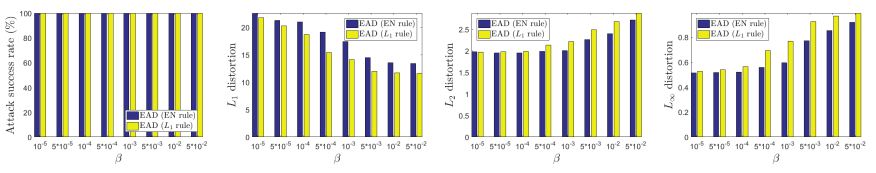
\includegraphics[width=1\textwidth]{assets/fig_02.png} 
    \caption{So sánh luật quyết định EN và $L_1$ trong EAD trên tập MNIST với nhiều tham số hiệu chỉnh $L_1$ $\beta$ (trường hợp trung bình). So sánh với luật EN cho cùng giá trị $\beta$} % Creates caption underneath graph
    \label{fig:fg_02}
\end{figure}

\begin{longtable}{l}
		\resizebox{\textwidth}{!}{
		\begin{tabular}{l|llll|llll|llll}
			\hline
			& \multicolumn{4}{c}{MNIST} & \multicolumn{4}{c}{CIFAR 10} & \multicolumn{4}{c}{ImageNet}\\
			\hline
			Attack method & ASR & $L_1$ & $L_2$ & $L_\infty$ & ASR & $L_1$ & $L_2$ & $L_\infty$ & ASR & $L_1$ & $L_2$ & $L_\infty$ \\
			\hline
			C\&W ($L_2$) & \textbf{100} & 22.46 & \textbf{1.972} & 0.514 & \textbf{100} & 13.62 & \textbf{0.392} & 0.044 & \textbf{100} & 232.2 & \textbf{0.705} & 0.03 \\
			FGM-$L_1$ & 39 & 53.5 & 4.186 & 0.782 & 48.8 & 51.97 & 1.48 & 0.152 & 1 & 61 & 0.187 & 0.007 \\
			FGM-$L_2$ & 34.6 & 39.15 & 3.284 & 0.747 & 42.8 & 39.5 & 1.157 & 0.136 & 1 & 2338 & 6.823 & 0.25 \\
			FGM-$L_\infty$ & 42.5 & 127.2 & 6.09 & 0.296 & 52.3 & 127.81 & 2.373 & 0.047 & 3 & 3655 & 7.102 & 0.014 \\
			I-FGM-$L_1$ & \textbf{100} & 32.94 & 2.606 & 0.591 & \textbf{100} & 17.53 & 0.502 & 0.055 & 77 & 526.4 & 1.609 & 0.054 \\
			I-FGM-$L_2$ & \textbf{100} & 30.32 & 2.41 & 0.561 & \textbf{100} & 17.12 & 0.489 & 0.054 & \textbf{100} & 774.1 & 2.358 & 0.086 \\
			I-FGM-$L_\infty$ & \textbf{100} & 71.39 & 3.472 & \textbf{0.227} & \textbf{100} & 33.3 & 0.68 & \textbf{0.018} & \textbf{100} & 864.2 & 2.079 & \textbf{0.01} \\
			EAD (EN rule) & \textbf{100} & \textbf{17.4} & 2.001 & 0.594 & \textbf{100} & \textbf{8.18} & 0.502 & 0.097 & \textbf{100} & \textbf{69.47} & 1.563 & 0.238 \\
			EAD ($L_1$ rule) & \textbf{100} & \textbf{14.11} & 2.211 & 0.768 & \textbf{100} & \textbf{6.066} & 0.613 & 0.17 & \textbf{100} & \textbf{40.9} & 1.598 & 0.293 \\
			\hline
		\end{tabular}} \\ 
		\caption{So sánh các tấn công trên các tập dữ liệu MNIST, CIFAR10 và ImageNet. ASR là tỷ lệ tấn công thành công (\%). Giá trị nhiễu trong bảng đo được trên giá trị trung bình của các mẫu thành công. EAD, C\&W và I-FGM-$L_\infty$ thu được các mẫu ít nhiễu nhất trên các chuẩn $L_1$,$L_2$,$L_\infty$ tương ứng. Kết quả đầy đủ được báo cáo trong tài liệu mở rộng.}
		\label{tab:tab_2}
\end{longtable}

Ở bảng \ref{tab:tab_1}, quá trình thuật toán tối ưu chạy để tìm ra mẫu đối nghịch cuối cùng giữa những mẫu đối nghịch thành công dựa trên hàm mất mát elastic-net trong $\{\mathbf{x}^{(k)}\}^I_{k=1}$, gọi là luật chọn elastic-net. Ngoài ra, có thể chọn mẫu đối nghịch cuối cùng sao cho $L_1$ nhỏ nhất, gọi là luật chọn $L_1$. Hình \ref{fig:fg_02} so sánh ASR và các nhiễu trung bình trên 2 luật chọn nói trên với các giá trị  khác nhau trên tập dữ liệu MNIST. Cả 2 luật chọn đều cho tỷ lệ thành công ASR $100\%$ với dải giá trị  rộng. Với cùng 1 giá trị , luật chọn $L_1$ cho ra các mẫu đối nghịch ít nhiễu $L_1$ hơn so với luật chọn EN, trong khi đó lại bị trả giá nhiều nhiễu hơn ở $L_2$, $L_{\infty}$ . Xu hướng tương tự cũng được quan sát thấy với CIFAR10 (kết quả đầy đủ với cả 2 tập dữ liệu MNIST và CIFAR có trong tài liệu mở rộng). Trong các thí nghiệm tiếp theo, nhóm tác giả báo cáo kết quả của EAD với 2 luật chọn và $\beta = 10^{-3}$, vì trên tập MNIST và CIFAR10 giá trị $\beta$ làm giảm nhiễu $L_1$ trong khi so sánh với $L_2$, $L_{\infty}$ với trường hợp $\beta = 0$ (nghĩa là không có hiệu chỉnh $L_1$).

